\graphicspath{{2D_QGNIW/code/plot_snap/figs/}}

The QG-NIW model was derived in \cite{XieVanneste_15}. It has been since further explored and expanded by \cite{WagnerYoung_15, WagnerYoung_16, AsselinYoung_19, Xie_20} and others. Here we will implement the two-dimensional version in \cite{RochaEtAl_18}. 

\section{The QG-NIW model}
We have the dimensional QG-NIW model (ignoring dissipation) from \cite[(2.6--8)]{RochaEtAl_18}:
\begin{align}
    &q = \nabla^2\psi + \frac{1}{f}\left[\frac{1}{4}\nabla^2|\phi|^2+\frac{i}{2}J(\phi^*,\phi)\right];\\
    &q_t + J(\psi,q) = 0;\\
    &\phi_t+J(\psi,\phi)+\phi\frac{i}{2}\nabla^2\psi-\frac{i}{2} \frac{N^2}{f m^2} \nabla^2\phi = 0.
\end{align}

\subsection{Nondimensionalization}
We make clear the true parameters dependence of the model by nondimensionalizing the model with:
\begin{align}
    &\phi \sim U_w = \epsilon^{-1} U_e\\
    &\psi \sim U_e L\\
    &L \sim L_e = k_e^{-1}\\
    &T \sim L/U_e
\end{align}
where
\begin{align}
    \epsilon = {U_e}/{U_w}\ll 1
\end{align}
indicated we are in the weak wave regime. Then we get (in the notation of \cite{Vallis_96a}):
\begin{align}
    &q = \nabla^2\psi + \frac{1}{f}\{\alpha\}\left[\frac{1}{4}\nabla^2|\phi|^2+\frac{i}{2}J(\phi^*,\phi)\right];\\
    &q_t + J(\psi,q) = 0;\\
    &\phi_t+J(\psi,\phi)+\phi\frac{i}{2}\nabla^2\psi-\frac{i}{2} \frac{N^2}{f m^2} \{\hbar\}\nabla^2\phi = 0\label{eq:QGNIW_eq3}
\end{align}
where we have the model depends on only two important nondimensional numbers, the wave amplitude:
\begin{align}
    &\alpha = \frac{U_e}{fL}\epsilon^{-2} = \text{Ro}\;\epsilon^{-2},
\end{align}
and the wave dispersivity:
\begin{align}
    &\hbar = \frac{N^2}{fm^2}\frac{1}{LU_e} = \frac{1}{\text{Ro}}\frac{N^2}{f^2 m^2 L^2}.
\end{align}
Note that Rossby number and the small parameter $\epsilon$ does not appear explicitly in the model. We only assume that they are small. Instead, their ratio appear as the wave amplitude $\alpha$. The distinguished limit assumptions in \cite{XieVanneste_15, WagnerYoung_15, WagnerYoung_16} is $\alpha = 1$. However, in \cite{RochaEtAl_18} it is allowed to vary in the $O(1)$ range. We also noticed that the Rossby number in \cite[Table 4]{RochaEtAl_18} is wrong. It should be $\approx 0.025$. However, the parameters that appear in the equations, $\hbar$ and $\alpha$, are correct.

The QG-NIW conserves energy and action. In particular we have the two energies (\cite[(3.2)]{RochaEtAl_18}):
\begin{align}
    &\mcal{K} = \frac{1}{2}|\nabla\psi|^2;\\
    &\mcal{P} = \frac{1}{4}\frac{N^2}{f^2m^2} |\nabla\phi|^2.
\end{align}
After the nondimensionalization, we have the total energy formula
\begin{align}
    \mcal{P} = \frac{1}{2}|\nabla\psi|^2+\{\alpha\hbar\}\frac{1}{4}\frac{N^2}{f^2m^2} |\nabla\phi|^2.
\end{align}
Note the introduction of the nondimensional numbers in from of the potential energy in the formula. They need to be accounted for in order for the total energy formula to be correct. 

\subsection{Separating the real and imaginary fields}
In the QG-NIW model, the $\phi$ field is complex while all other fields are real. If we put the equation as is into Dedalus, all fields must be complex, with the real fields having zero imaginary parts. However, for DFT, real-input require roughly half the computation time of complex-input. This will potentially degrade performance\footnote{See a discussion with the Dedalus developer in \url{https://groups.google.com/u/1/g/dedalus-users/c/habu7iKCCWc/m/mNNGPqLuAwAJ}}. To address this issue, we write the equation in term of the real and imaginary parts of $\phi$. Now all fields can be real. We write the nondimensional equations:
\begin{align}
    &q = \nabla^2\psi + \frac{1}{f}\{\alpha\}\left[\frac{1}{4}\nabla^2(\phi_r^2+\phi_i^2))-J(\phi_r,\phi_i)\right];\\
    &q_t + J(\psi,q) = 0;\\
    &\phi_{r,t}+J(\psi,\phi_r)-\frac{\phi_i}{2}\nabla^2\psi+\frac{\hbar}{2}\nabla^2\phi_i = 0\\
    &\phi_{i,t}+J(\psi,\phi_i)+\frac{\phi_r}{2}\nabla^2\psi-\frac{\hbar}{2}\nabla^2\phi_r = 0
\end{align}

% \section{The Lamb–Chaplygin dipole simulation}

\section{2D turbulence modified by NIW}
\subsection{The parameters}
We use the set-up of \cite[Tabel 4 \& \S 4.2]{RochaEtAl_18}. We pick the nondimensional parameters
\begin{align}
    \alpha = 0.1 \qdt{and} \hbar = 1.
\end{align}
Note that since we have the energy containing scale nondimensionalized to be 1, we have $k_e = 2\pi$ and the domain size to be 10. The $k_e$ value is worth noting when comparing to the results of \cite{RochaEtAl_18}.

We use the same hyper-diffusivity as \cite[(2.9a,b)]{RochaEtAl_18}. We pick $\kappa_e=\nu_w = 8\times 10^{-7}$. This is roughly the same dissipation as the numbers in \cite[Tabel 4]{RochaEtAl_18} as in our nondimensionalization and $512^2$ resolution.

\subsection{The balanced flow generation}
We run a 2D Euler simulation to generate the background mean flow using the code in Chapter \ref{chap:2DEuler}. We start the energy according to \cite[(4.2)]{RochaEtAl_18} and pick the roughly correct amplitude so that the resulting field matches the amplitude of the \cite{RochaEtAl_18} paper. We let the system evolve and Figure \ref{fig:PVbalanced} the resulting balanced flow. It looks similar to Figure 5(a) of \cite{RochaEtAl_18}. 
\begin{figure}[h]
    \centering
    % 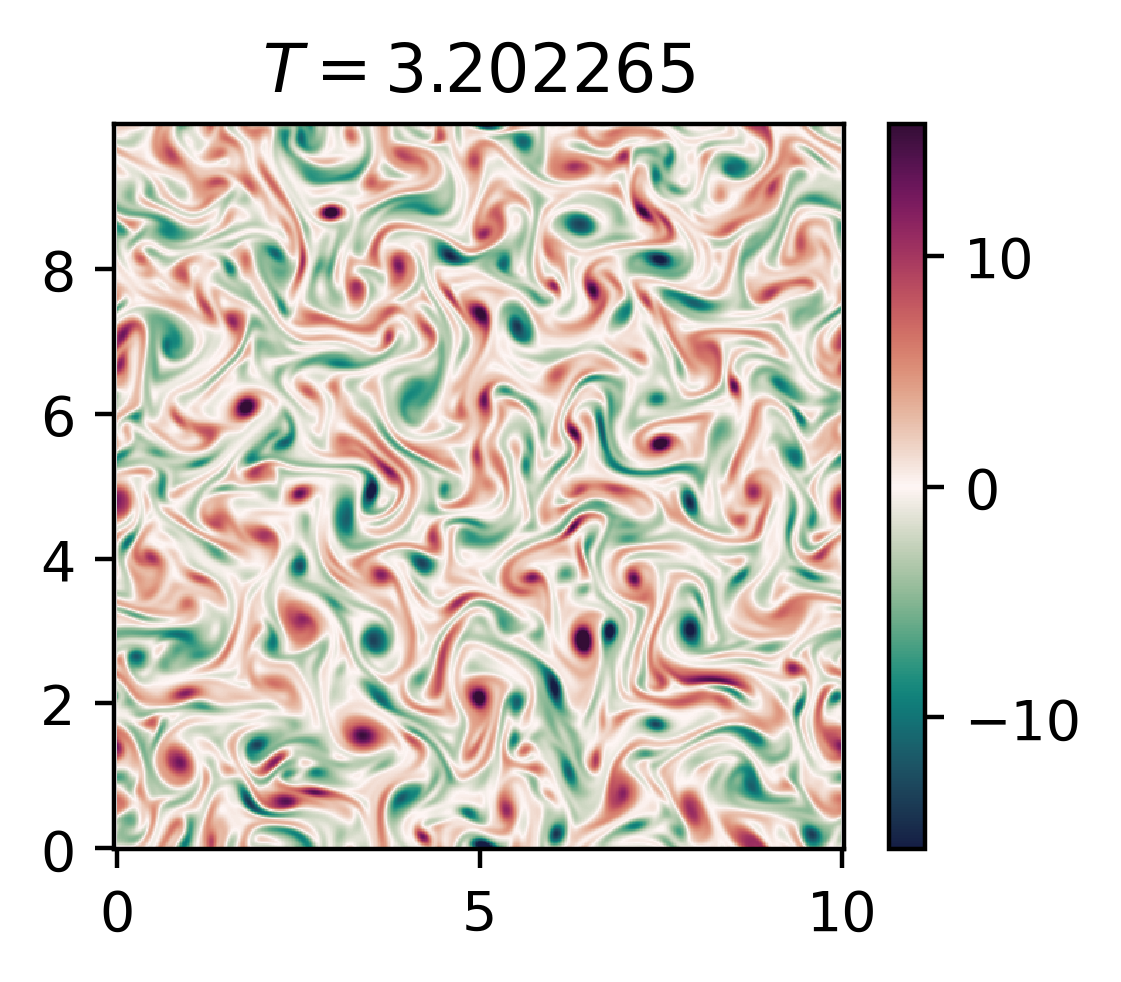
\includegraphics{PVbalanced}
    \caption{Left: the entire PV field. Right: a zoomed in picture of $(1/2)^2$ of the domain, with time and PV scaled so that to match the numbers of \cite{RochaEtAl_18}.}
    \label{fig:PVbalanced}
\end{figure}

\subsection{QG-NIW Simulation}
We simulate the QG-NIW model by adding in a wave field of
\begin{align}
    \phi = \frac{1}{\sqrt{2}}(1+i)
\end{align}
on top of the above PV field. Figure \ref{fig:QGNIW_t1} shows the result. They compare well with Figure 5 of \cite{RochaEtAl_18}.
\begin{figure}[h]
    \centering
    % 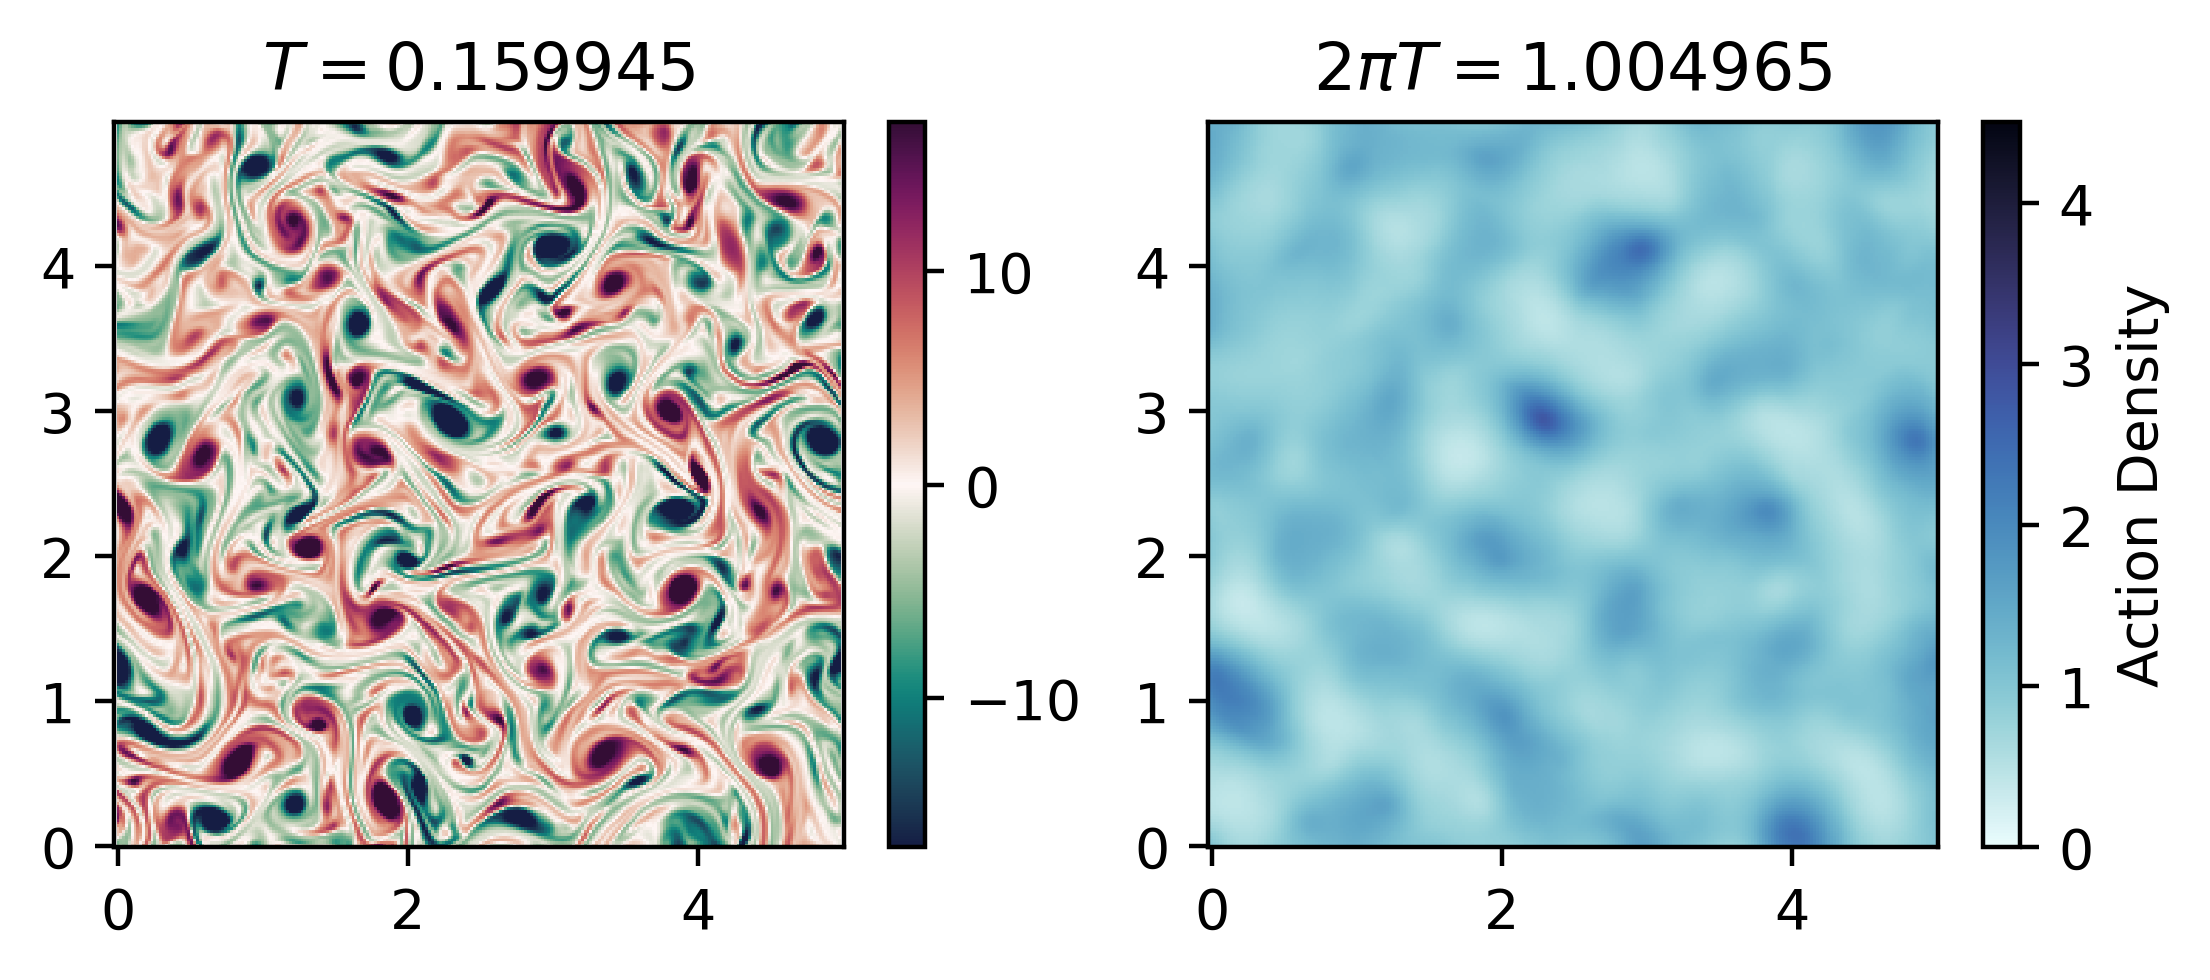
\includegraphics{QGNIW_t1}
    % 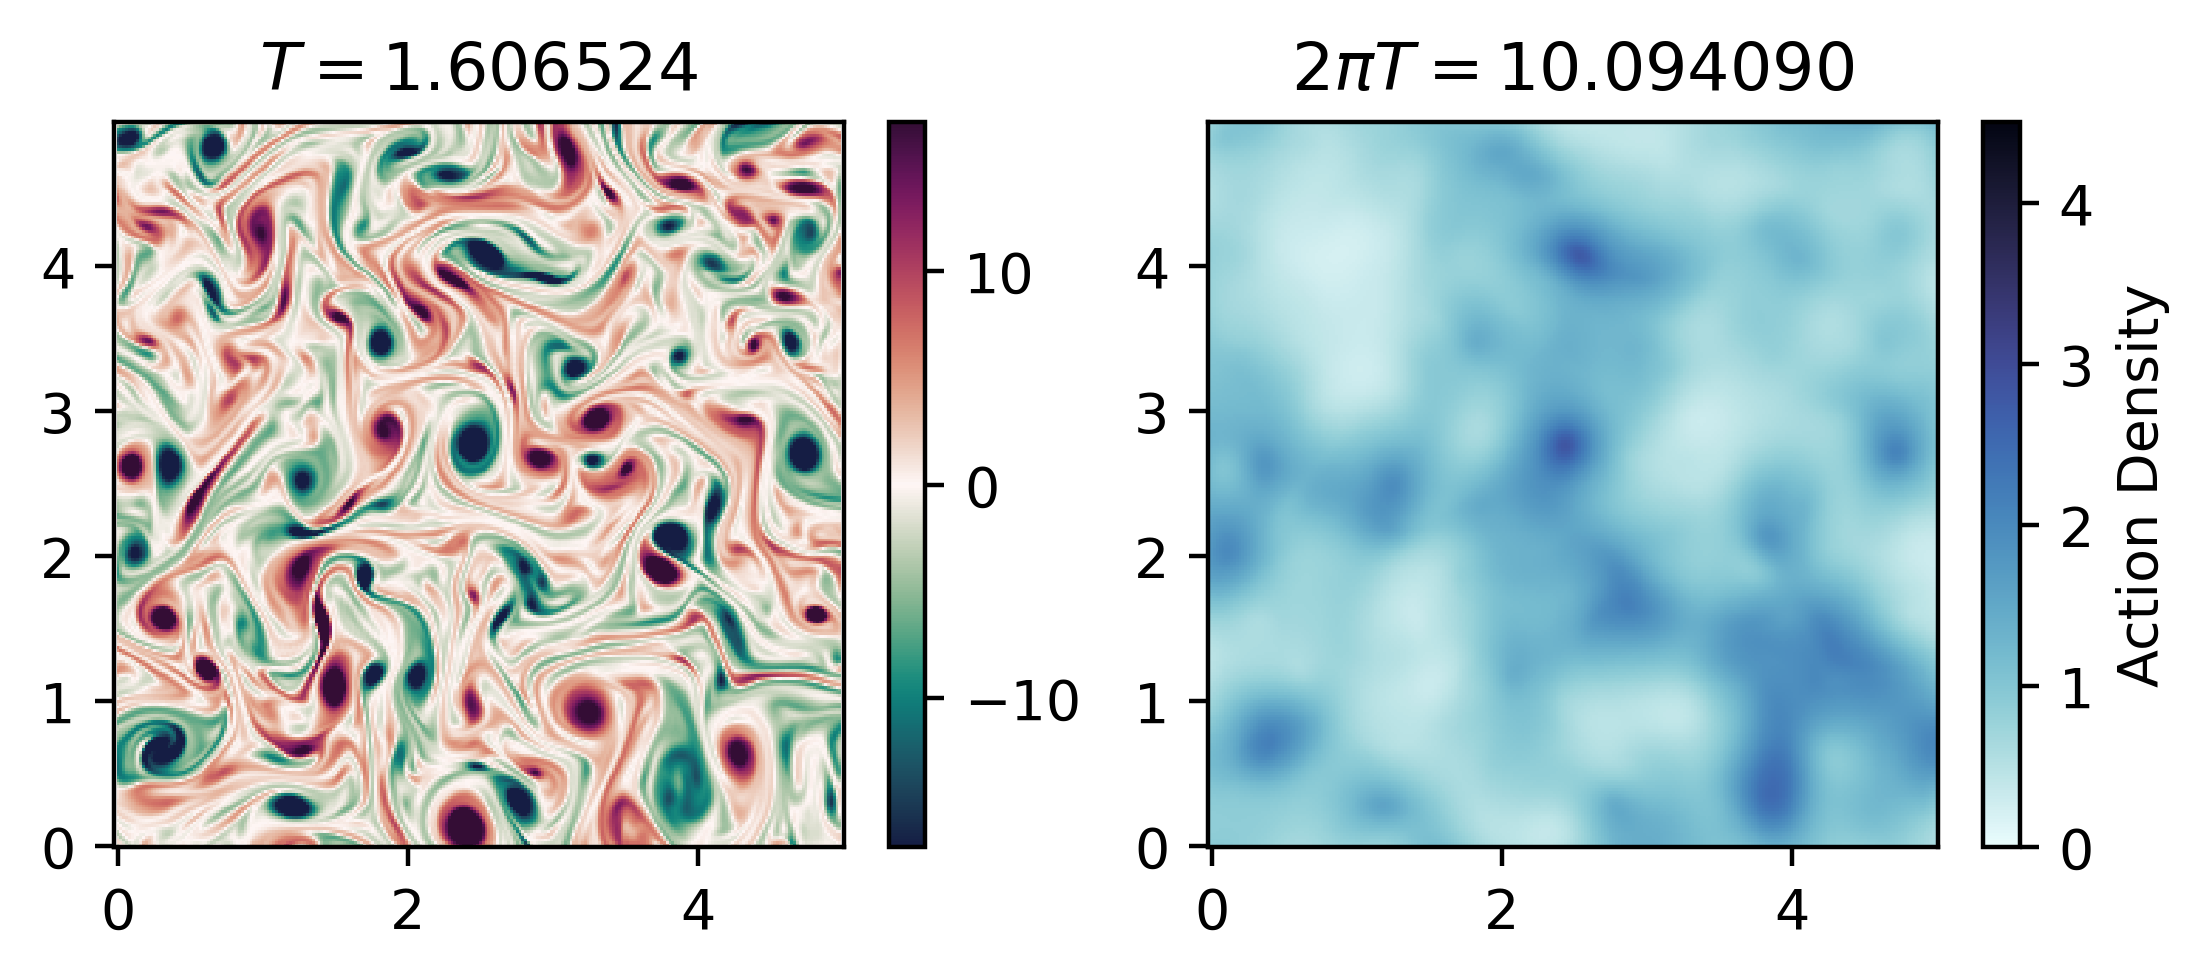
\includegraphics{QGNIW_t10}
    \caption{}
    \label{fig:QGNIW_t}
\end{figure}

\section{Some comments}
\subsection{The IMEX time-stepper and YBJ\textsuperscript{+} equation}
We use the 3rd-order 4-stage DIRK+ERK scheme (\texttt{RK443}) for time integration \parencite[Sec 2.8]{AscherEtAl_97}. It enjoys the property that the stability region of RK4 includes a portion of the imaginary axis. This is crucial for the stable evolution of the refraction term in the $\phi$ equation. It is also an implicit-explicit (IMEX) method that treat the stiff linear terms implicitly. This include the dispersion term in \eqref{eq:QGNIW_eq3}. Therefore we can stably simulate the original QG-NIW system as written in \cite{XieVanneste_15} and \cite{RochaEtAl_18} at high resolution. \cite{AsselinYoung_19} has modified the dispersion term in their YBJ\textsuperscript{+} equation so that the wave frequency asymptotes to twice the inertial frequency $2f$, instead of growing as $k^2$. They cite this allows explicit time-stepping of their equations. While this is true, we think this improvement is inconsequential since all turbulence simulation needs small scale dissipation, which is as stiff or stiffer than $k^2$. We have to treat stiff linear terms implicitly anyway. 

However, the IMEX is an imperfect solver for the QG-NIW system. We observe that the action is not monotonically decreasing in our simulation. This might be because the implicit treatment of the dispersion term allows for stable integration, but it does not guarantee conservation of quadratic quantities. \cite{RochaEtAl_18} uses an exponential integrator, which treat the linear terms exactly. It is a more ideal method, but is not yet implemented in Dedalus.

The YBJ\textsuperscript{+} equation in \cite{AsselinYoung_19} has other benefits of course. To simulate it in Dedalus, we need to be able to define an unusual linear operator, $\mcal{P}$ in \cite[(3.2)]{Xie_20}. It is currently unclear to us on how to do this. For more see the comments in Section  \ref{sec:ded_want_linop}.

With all these caveat, we do not recommend using Dedalus to simulation the QG-NIW system at this time. We recommend a custom implementation using exponential time integrator\footnote{A 1D example is \url{https://github.com/Empyreal092/MMT_Public}.}.

\subsection{Another implementation in v2}
A Dedalus solver for QG-NIW also exists using Dedalus version 2 \parencite{Conn_2023}. The current implementation uses the more recent version 3, which is being actively updated. For example, Dedalus only recently (June 25, 2023)\footnote{\url{https://github.com/DedalusProject/dedalus/commit/d3843a7394e06c05bf56ba2710723e42ba19ef39}\;} allowed restart with partial data in v3 (the \verb|allow_missing| flag in \verb|solver.load_state|). Our version adaptively changes the timestep, therefore is more efficient. Their version uses a lower over RK method, which requires very small timestep for stability, and might suffer the same lack of action conservation. 
